\documentclass[e4_tp1_main.tex]{subfiles}
\begin{document}

\section{DCM y Eficiencia}


Para llevar el circuito del inciso anterior a modo discontinuo se dismunuy\'o la corriente de salida a $I_o=10mA$.  Para una tensi\'on de salida $V_o=3.3V$ con $\Delta V_o =5\%$, debimos modificar el duty cycle a $D_{real}=0.35$.


\subsection*{a) Curvas simuladas}

\begin{figure}[H]
\centering
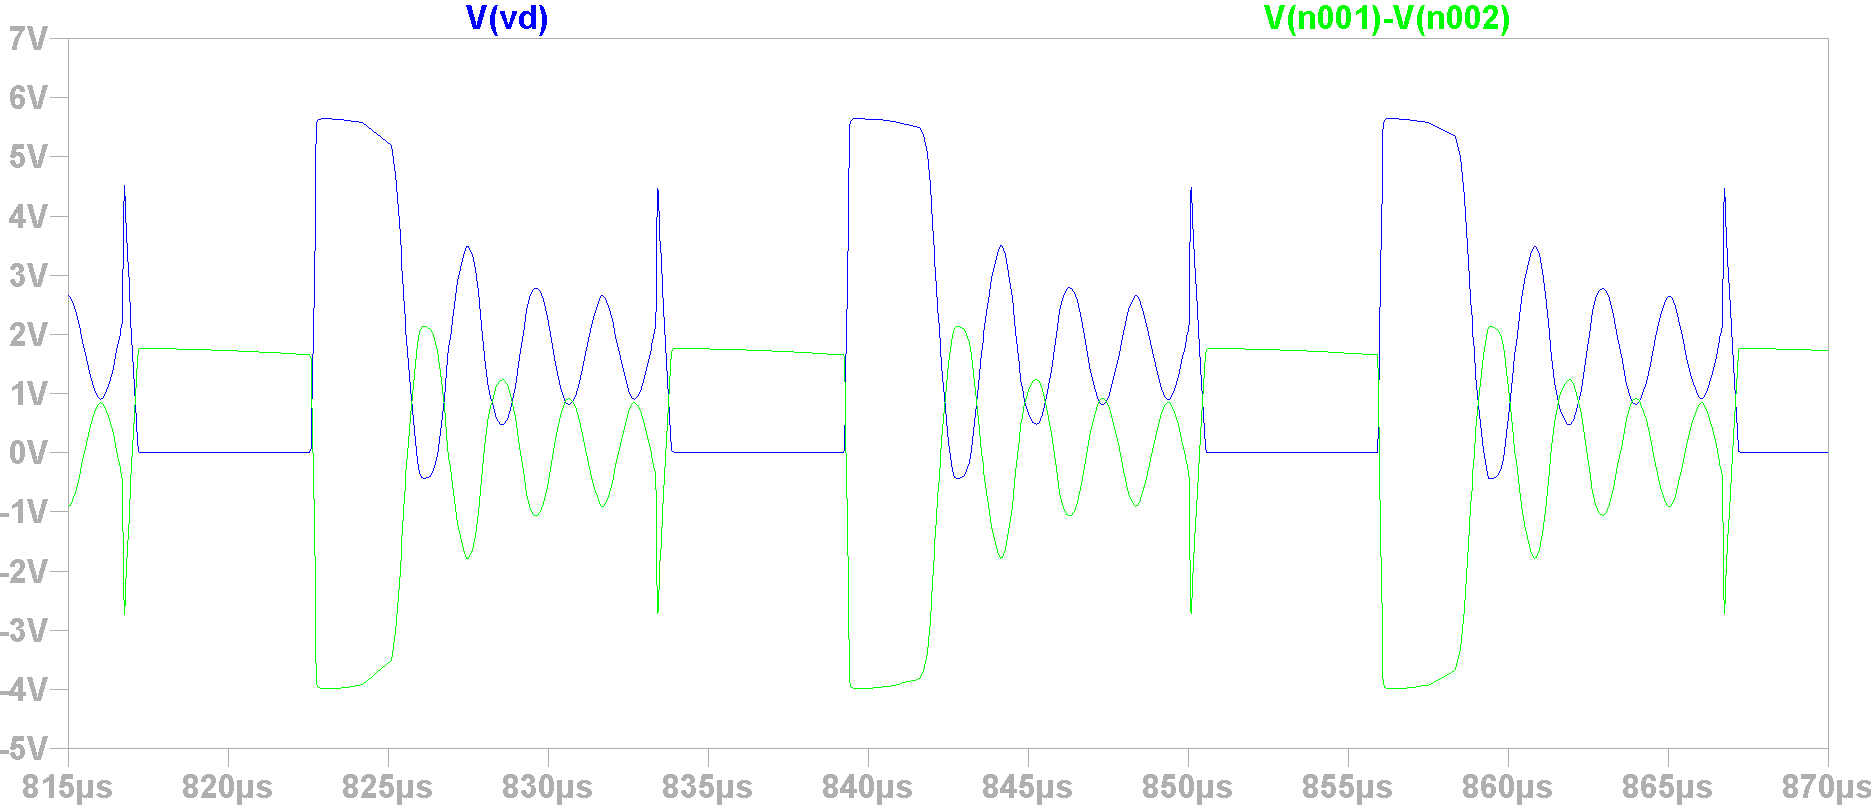
\includegraphics[width=0.9\linewidth]{Imagenes/Punto4/SW&VL}
\caption{Simulación Sw(azul) y VL(verde)}
\end{figure}

\begin{figure}[H]
\centering
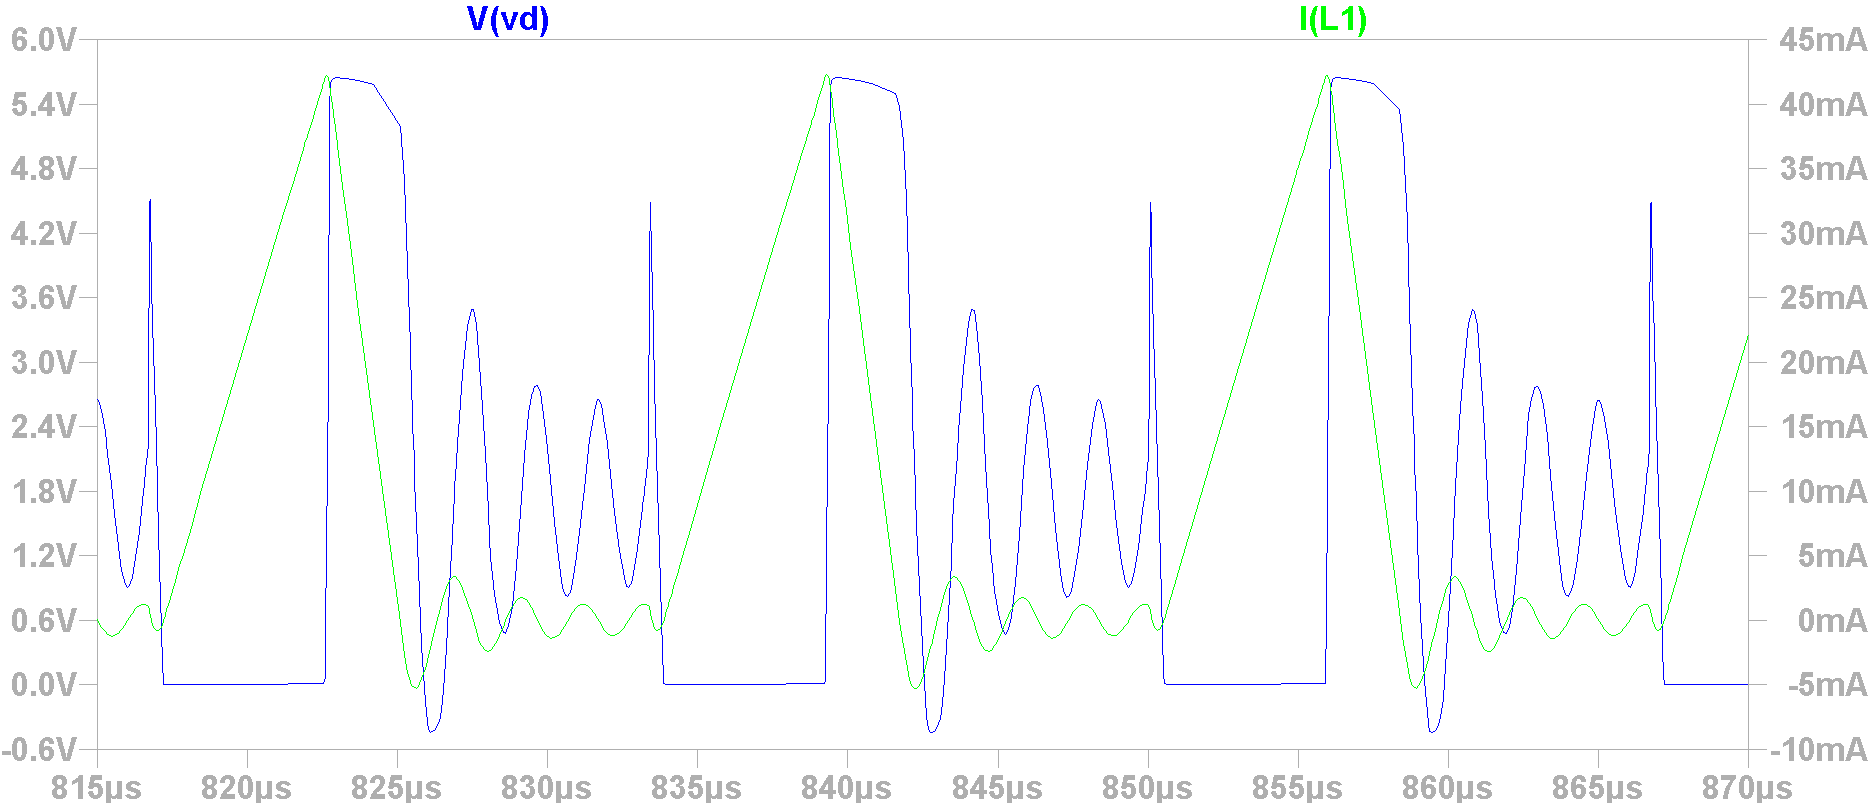
\includegraphics[width=0.9\linewidth]{Imagenes/Punto4/SW&IL}
\caption{Simulación Sw(azul) y IL(verde)}
\end{figure}

\begin{figure}[H]
\centering
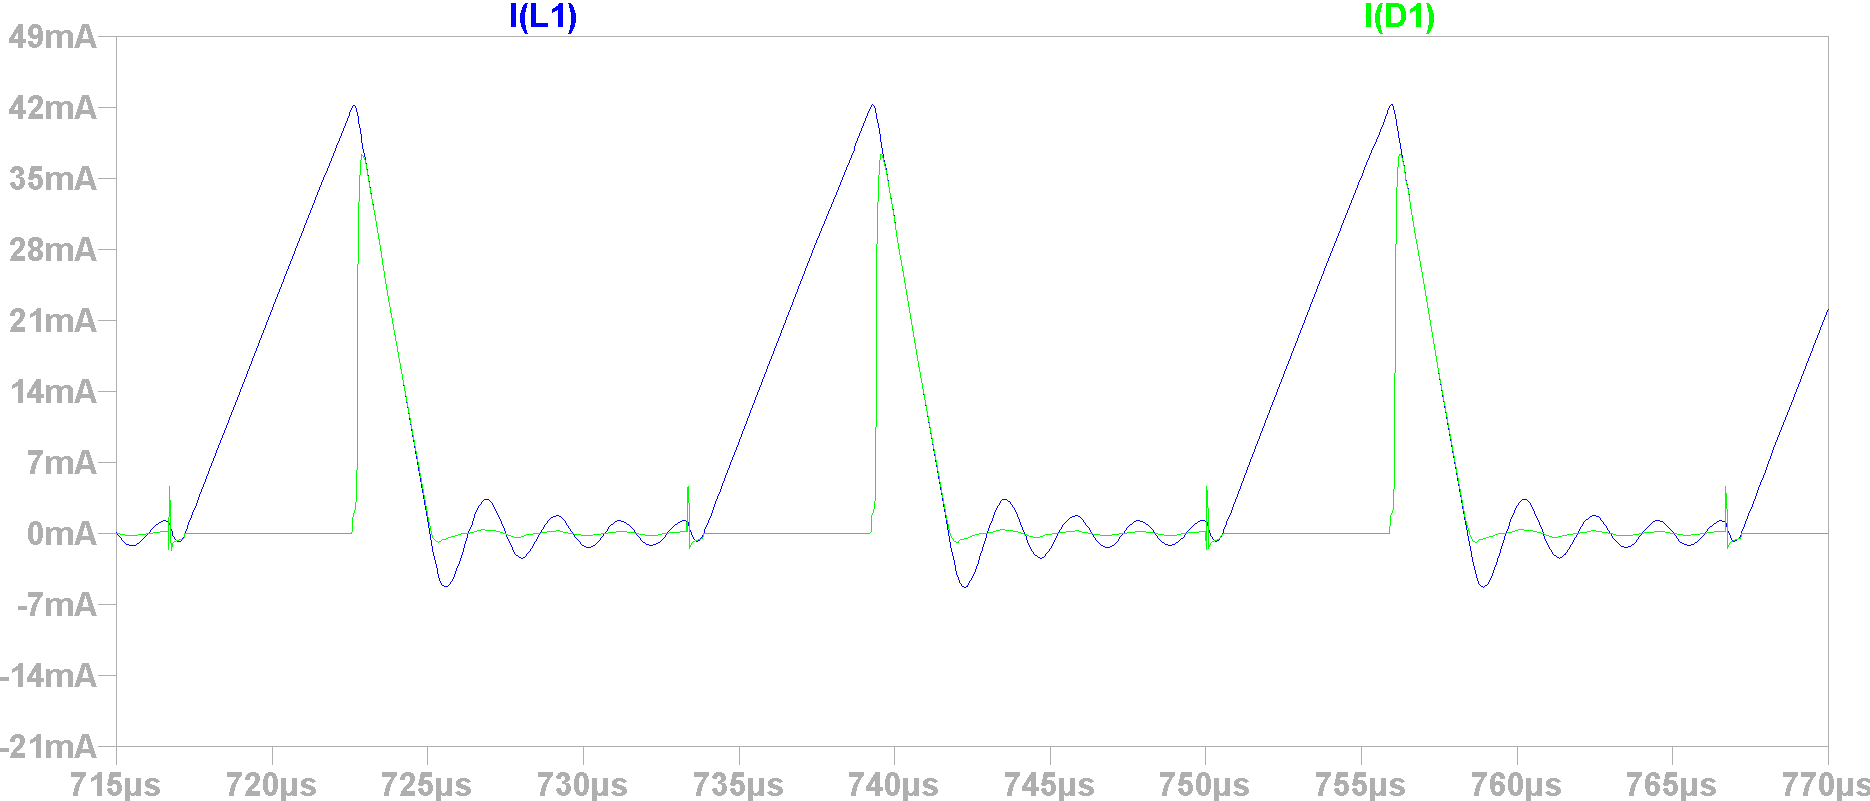
\includegraphics[width=0.9\linewidth]{Imagenes/Punto4/IL&ID}
\caption{Simulación IL(azul) y ID(verde)}
\end{figure}

\begin{figure}[H]
\centering
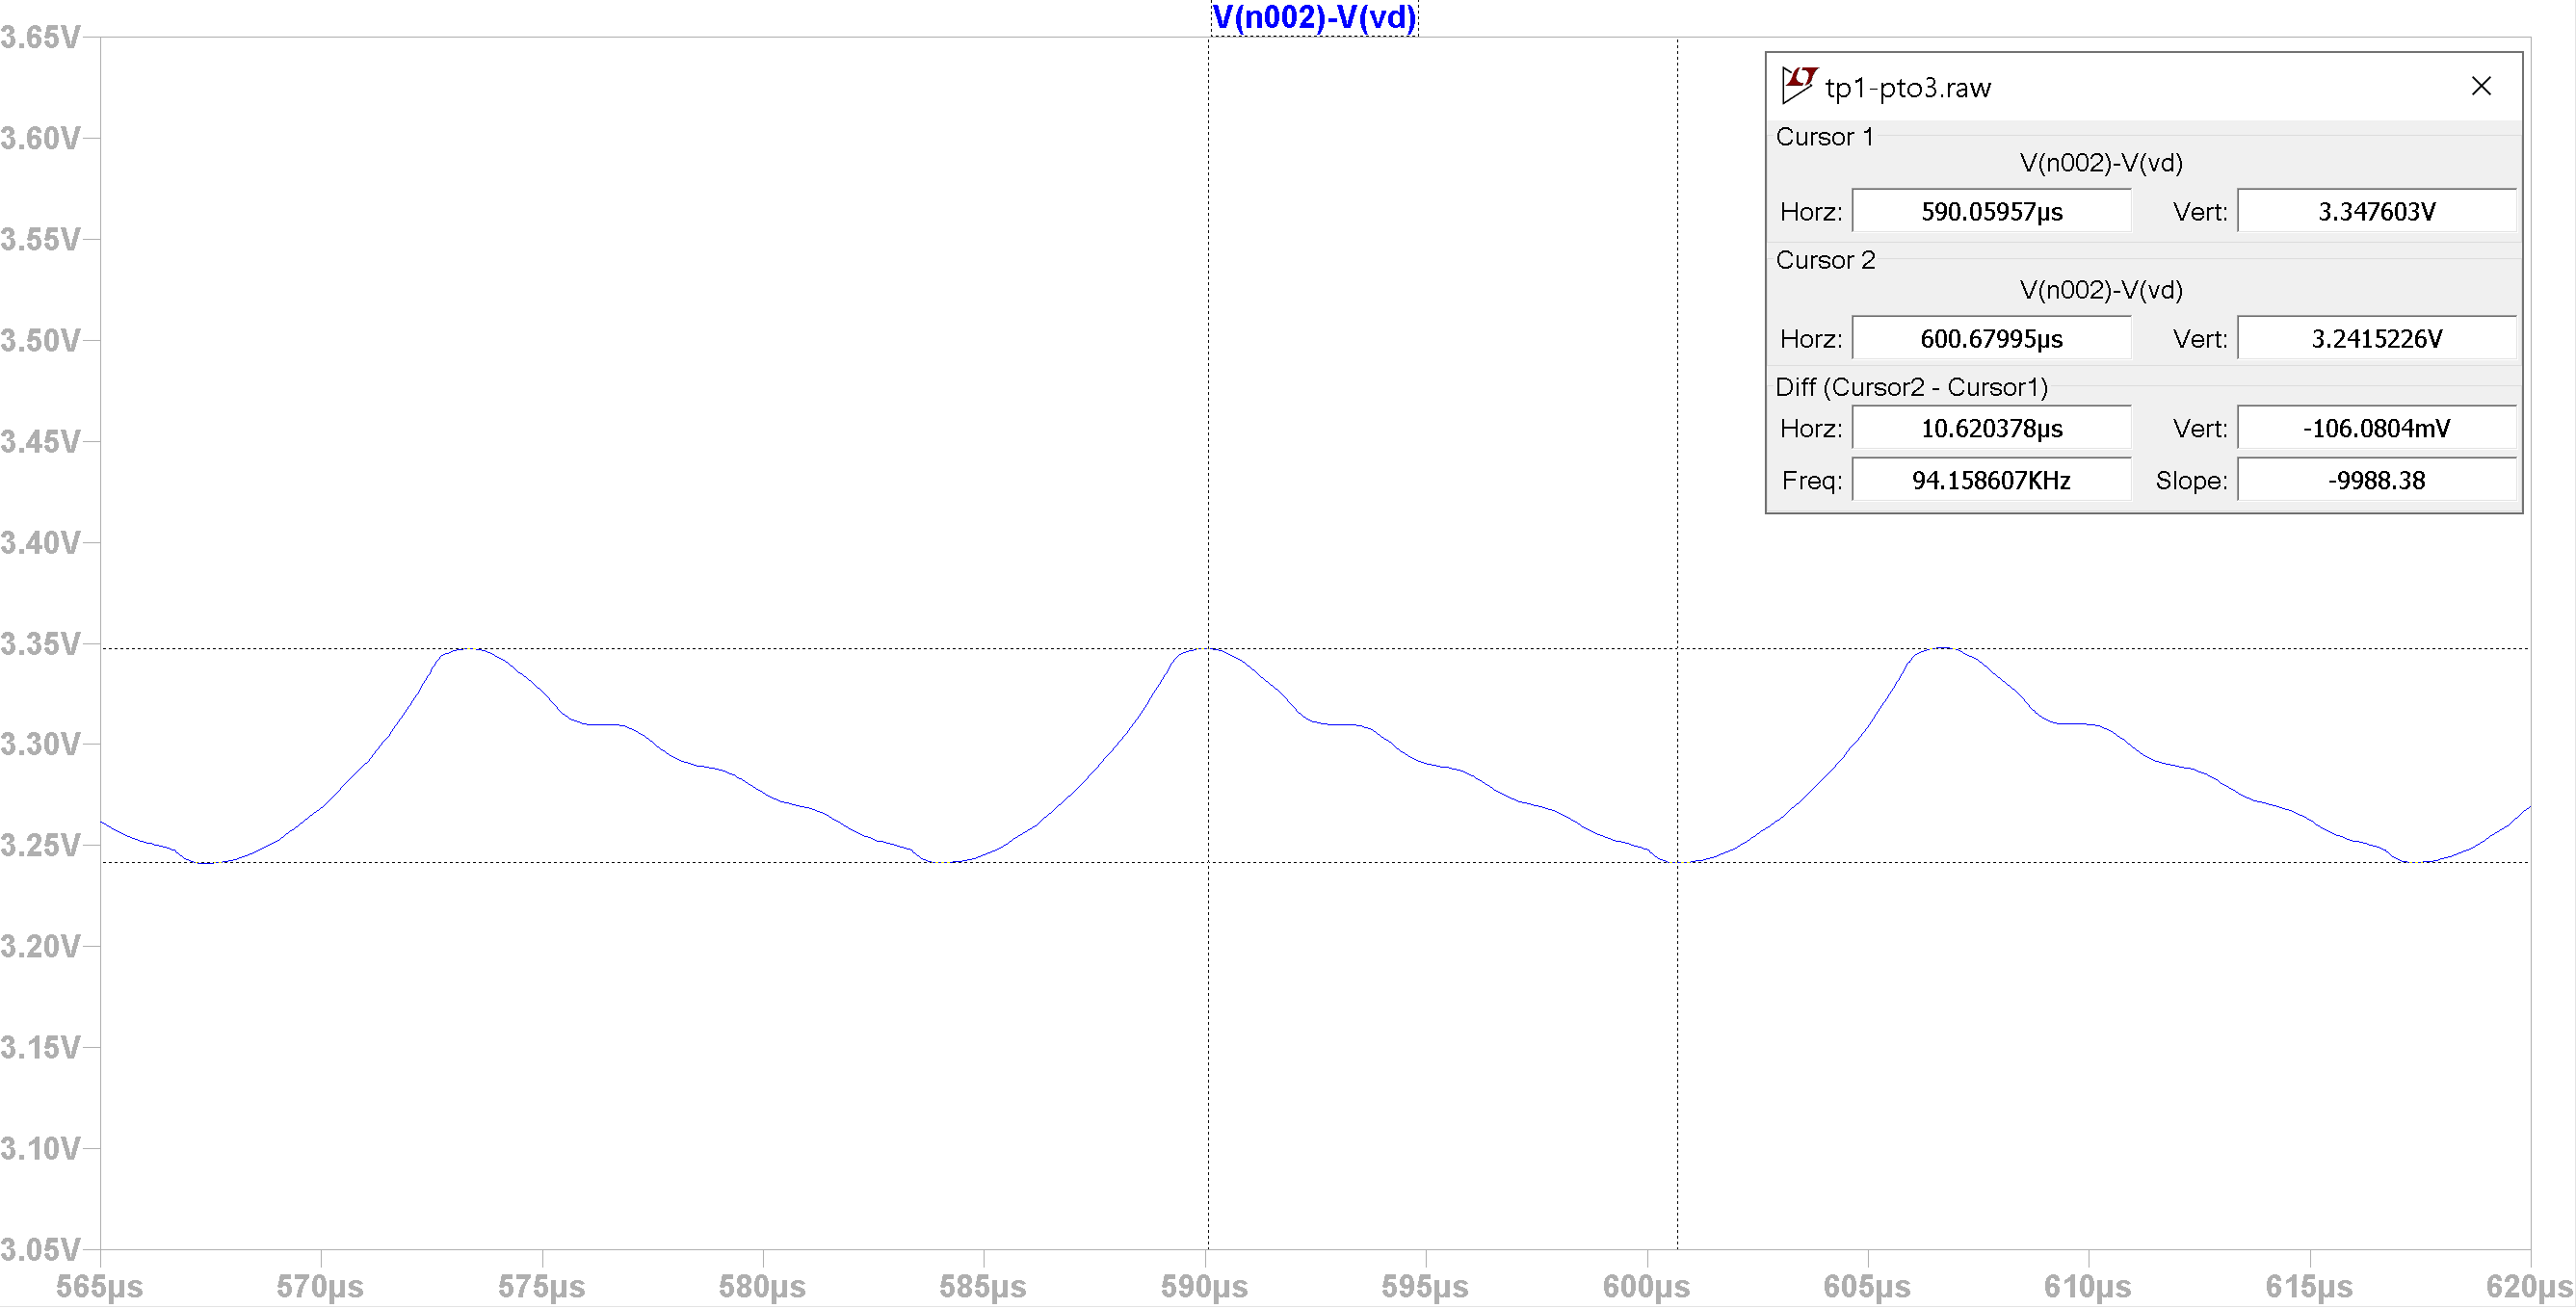
\includegraphics[width=0.9\linewidth]{Imagenes/Punto4/Vo-D=0,35.PNG}
\caption{Simulación $V_o$}
\end{figure}

\subsubsection*{1- Comparaciones y observaciones}

Al pasar el circuito al modo discontinuo, tenemos que tanto el diodo como el transistor tienen una mayor pendiente en la corriente, teniendo que poder soportar una mayor proporción de corriente respecto a la que circula por la carga que lo que observamos en el modo continuo. Por otro lado, esto permitió disminuir el duty para obtener la misma $V_o$.
\par
Cuando el transistor se apaga, $V_{ds}$ se mantiene estable mientras la bobina se descarga. Cuando ésta se termina de descargar y la rama queda sin corriente, el nodo de drain queda en alta impedancia, por lo que las capacidades de salida del MOS y las parásitas del diodo (que está sin polarizar) intercambian energía, produciendo las oscilaciones sobre dicho nodo, como se observa en la primer figura. Éstas se ven reflejadas en la corriente de la bobina, que en lugar de mantenerse nula permite notar unas pequeñas oscilaciones, que también pasan a observarse en la corriente del capacitor. Como la corriente media en el capacitor es nula, y la tensión sobre él no puede cambiar abruptamente, prácticamente no afecta en forma significativa a la tensión de salida.
\par
Al haber disminuido la corriente de carga (aumentando la resistencia), el ripple por efecto de la ESR del capacitor disminuye, por lo que el ripple final resultante a la salida es menor en comparación al circuito en modo continuo.


\subsubsection*{2- Potencia CCM y DCM - Comparaciones}

Se tomaron también capturas haciendo foco en los tiempos de conmutación.

\begin{figure}[H]
\centering
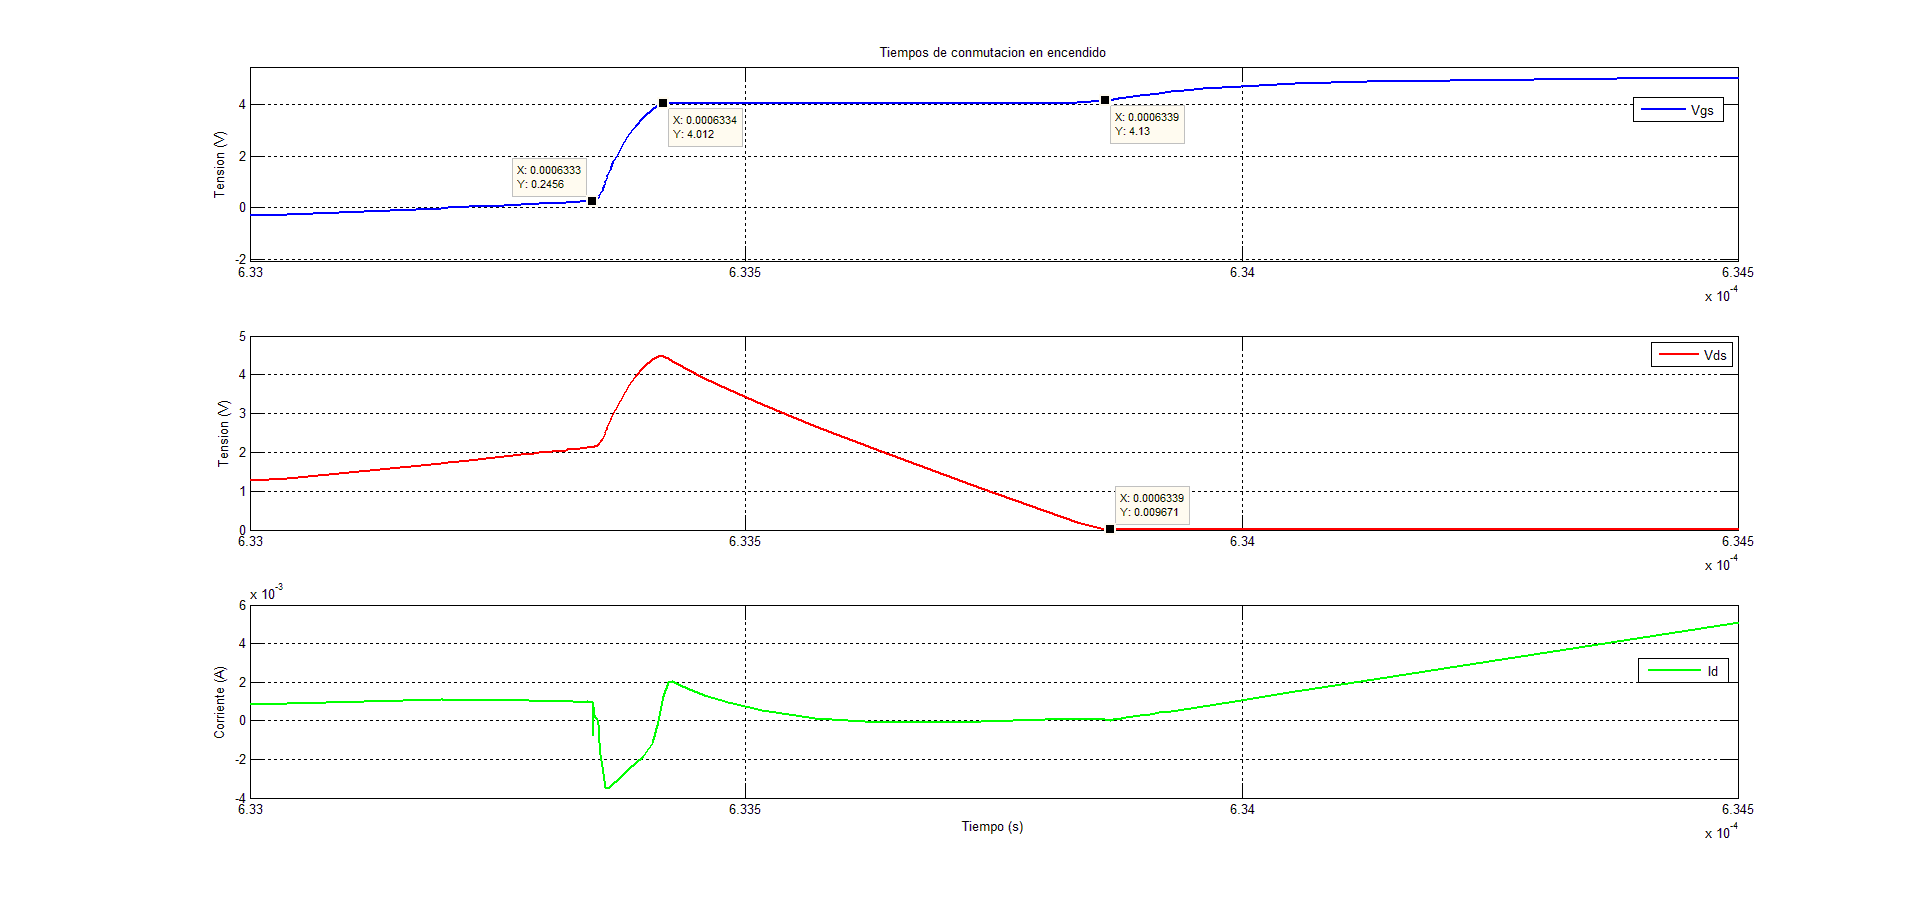
\includegraphics[width=1\linewidth]{Imagenes/Punto4/tiempos_encendidoX.png}
\caption{Curvas de encendido simulado}
\end{figure}

Al tener tiempos de conmutación menores en el encendido respecto al circuito en modo continuo, las pérdidas de potencia en el encendido resultan menores.

\begin{figure}[H]
\centering
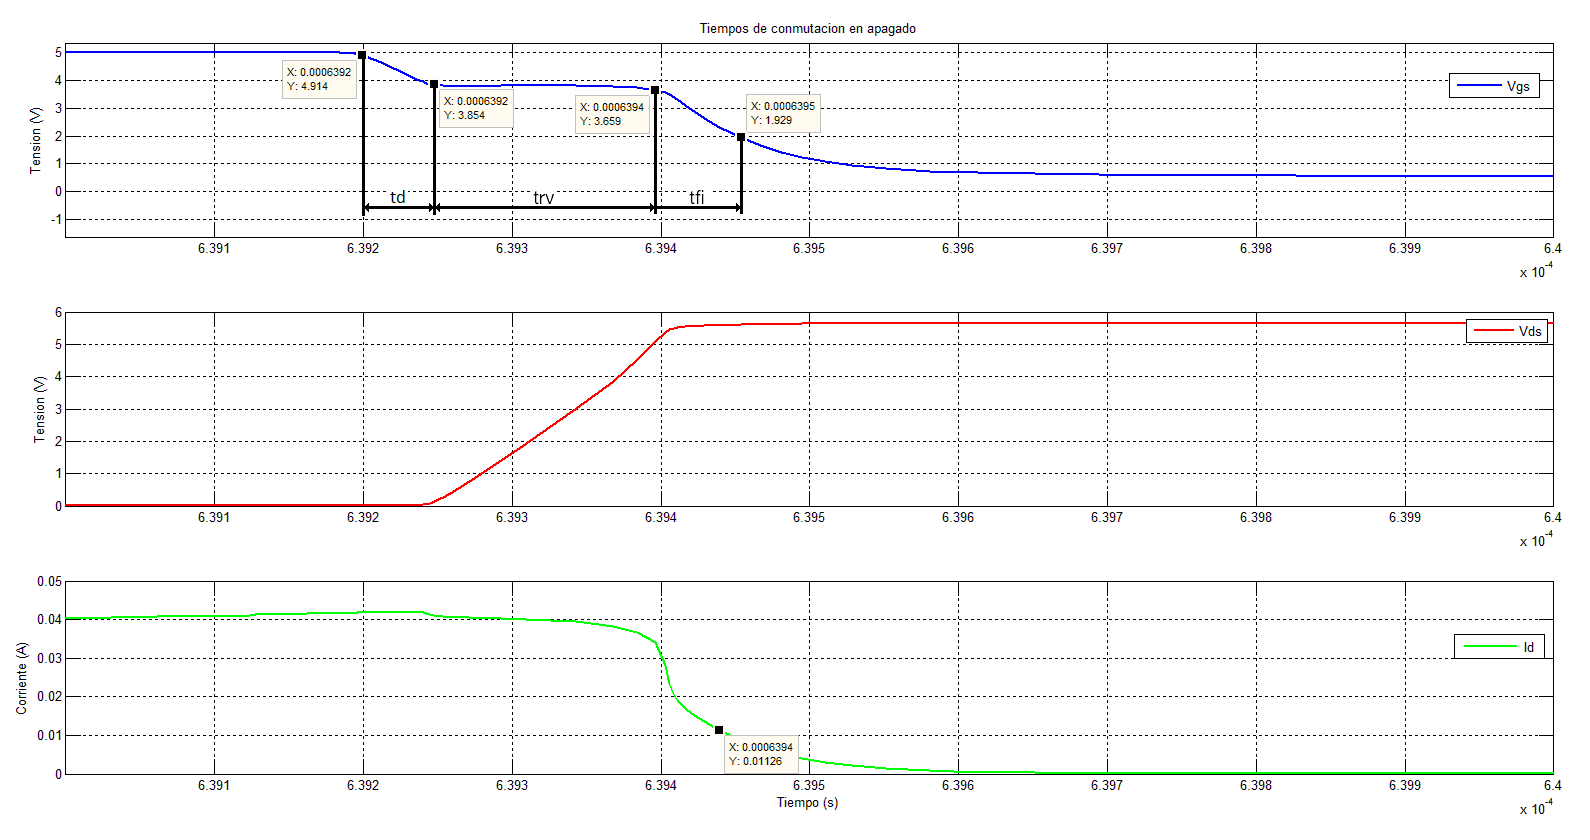
\includegraphics[width=1\linewidth]{Imagenes/Punto4/tiempos_apagadoX.png}
\caption{Curvas de apagado simulado}
\end{figure}

Por otra parte, los tiempos de conmutación del apagado son mayores, por lo que las pérdidas de potencia en el apagado son, entonces, mayores que en modo continuo.

\newpage
\end{document}